\chapter{Dynamics of humanoid locomotion}
Intro. Robot walks by exchanging forces with the environment. Dynamic balance, contacts. Simplified models and contact equilibrium.

\section{Lagrangian dynamics}
\label{sec:lagrangian-dynamics}
Define configuration of the robot:
\begin{equation*}
    \ddot{\bm{q}} =
    \begin{bmatrix}
        \bm{q}_b \\ \bm{q}_j
    \end{bmatrix} \in \mathrm{SE}(3) \times \mathrm{SO}(2)^{n_j}
\end{equation*}

Equations of motion
\begin{equation}
    \begin{bmatrix}
        \bm{M}_u \\ \bm{M}_a
    \end{bmatrix} \ddot{\bm{q}} +
    \begin{bmatrix}
        \bm{c}_u(\bm{q}, \dot{\bm{q}}) \\
        \bm{c}_a(\bm{q}, \dot{\bm{q}}) \\
    \end{bmatrix} =
    \begin{bmatrix}
        \bm{0} \\ \bm{\tau}
    \end{bmatrix} +
    \sum_{k=1}^{K}
    \begin{bmatrix}
        \bm{J}_{k, u}^T \\ \bm{J}_{k, a}^T
    \end{bmatrix}
    \bm{f}_k
    \label{eq:equation-of-motion-humanoids}
\end{equation}

Contact forces inside the friction cone to avoid slipping

A contact force $\bm{f}_k$ is \textit{feasible} if it lies in the friction cone $\mathcal{C}_k$ directed by the contact normal $\bm{n}_k$:
\begin{equation}
    \label{eq:feasible-contact-force}
    \| \bm{f}_k - (\bm{f}_k \cdot \bm{n}_k) \bm{n}_k \|_2 \le \mu_k (\bm{f}_k \cdot \bm{n}_k)
\end{equation}
with $\mu_k$ static friction coefficient.

In the following we will assume that there always exists joint torques
$\bm{\tau}$ that realize the actuated part of eq.
\eqref{eq:equation-of-motion-humanoids}.

\section{Centroidal dynamics}
The above hypothesis allows as to focus on the unactuated part of the equation
\eqref{eq:equation-of-motion-humanoids}, and define the
\textit{centroidal dynamics} \cite{Orin2013CentroidalDynamics} of the humanoid:
\begin{equation}
    \label{eq:centroidal-dynamics}
    \begin{bmatrix}
        m \ddot{\bm{p}}_C \\ \dot{\bm{L}}_C
    \end{bmatrix} =
    \begin{bmatrix}
        m \bm{g} \\ \bm{0}
    \end{bmatrix} +
    \sum_{k=1}^K
    \begin{bmatrix}
        \bm{f}_k \\ (\bm{p}_C - \bm{p}_k) \times \bm{f}_k
    \end{bmatrix},
\end{equation}
where $m$ is the total mass of the robot, $\bm{p}_C$ is the position of its
center of mass (CoM),
$\bm{g} = (0 \; 0 \; {-g})^T$ is the gravity vector ($g=9.81$~[m/s$^2$]), $\bm{f}_k$ is the contact force
applied at a point with coordinates $\bm{p}_k$ over a contact surface with normal
$\bm{n}_k$, $K$ is the total number of contacts, and $\bm{L}_c$ is the angular
momentum of the robot taken at the CoM.

Let us define the \textit{gravito-inertial wrench} taken at point $O$ as
\begin{equation}
    \label{eq:gravito-intertial-wrench}
    \bm{w}_O^{\rm gi}
    =
    \begin{bmatrix}
        \bm{f}^{\rm gi}\\
        \bm{\tau}_O^{\rm gi}
    \end{bmatrix}
    =
    \begin{bmatrix}
        m \bm{g} - m \bm{\ddot{p}}_C \\
        (\bm{p}_C - \bm{p}_O) \times (m \bm{g} - m \bm{\ddot{p}}_C) - \bm{\dot{L}}_C
    \end{bmatrix}.
\end{equation}

Similarly, the \textit{contact wrench} $\bm{w}_O$ can be defined as
\begin{equation}
    \label{eq:contact-wrench}
    \bm{w}_O^{\rm c}
    =
    \begin{bmatrix}
        \bm{f}^{\rm c} \\
        \bm{\tau}_O^{\rm c}
    \end{bmatrix}
    =
    \sum_{k=1}^K
    \begin{bmatrix}
        \bm{f}_k\\
        (\bm{p}_k - \bm{p}_O) \times \bm{f}_k
    \end{bmatrix}.
\end{equation}

Note that the centroidal dynamics \eqref{eq:centroidal-dynamics} can be
rewritten as a sum of the two above wrenches
\begin{equation}
    \bm{w}_O^{\rm gi} + \bm{w}_O^c = 0.
\end{equation}

\section{Zero-tilting moment point}
\label{sec:zero-tilting-moment-point}
Consider the gravito-inertial wrench defined in \ref{eq:gravito-intertial-wrench}. Zero-tilting moment points (ZMPs) are points $Z$ where the moment of the contact wrench aligns with the normal $\bm{n}$ of the contact surface \cite{SardainBessonnet2004}, i.e.,
\begin{equation}
    \label{eq:zmp-non-tilting-condition}
    \bm{\tau}_Z^{\rm gi} \times \bm{n} = \bm{0},
\end{equation}
which, using Varignon formula\footnote{A screw $\bm{w}_O =
(\bm{f},\bm{\tau}_O)$ represents the generalized force acting on a rigid body
\cite{Featherstone2007RigidBodyDynamicsAlgorithms},
and it is composed by a linear force $\bm{f}$ passing through $O$, together with the
total moment $\bm{\tau}_O$ about $O$. That total moment around any other point
$A$ can be computed using Varignon formula as $\bm{\tau}_A=\bm{\tau}_O+\bm{f}\times(\bm{p}_A-\bm{p}_O)$.}, can be rewritten as
\begin{equation*}
    \left(\bm{\tau}_O^{\rm gi} + (\bm{p}_O - \bm{p}_Z) \times \bm{f}^{\rm gi}\right) \times \bm{n} = \bm{0},
\end{equation*}
which, developing the triple cross product\footnote{The triple cross product
between three vectors $\bm{a}, \bm{b}, \bm{c} \in \mathrm{R}^n$ is defined as
the cross product of the vector $\bm{a}$ with the cross product of the other
two: $\bm{a}\times(\bm{b}\times\bm{c})=(\bm{a}\cdot\bm{c})\bm{b}-
(\bm{a}\cdot\bm{b})\bm{c}$. Note that, since the cross product is anticommutative,
the following holds:
($\bm{a}\times\bm{b})\times\bm{c}=-(\bm{c}\cdot\bm{b})\bm{a}+
(\bm{c}\cdot\bm{a})\bm{b}$.}, the above equation becomes
\begin{equation}
    \bm{\tau}_O^{\rm gi} \times \bm{n} - (\bm{n} \cdot \bm{f}^{\rm gi}) (\bm{p}_O - \bm{p}_Z) - \left(\bm{n} \cdot (\bm{p}_O - \bm{p}_Z)\right) \bm{f}^{\rm gi} = \bm{0}.
\end{equation}

Assuming that a point $Z$ lies on a plane with normal $\bm{n}$ intersecting the point $O$, i.e. $Z \in \Pi(O, n)$, the term $\bm{n} \cdot (\bm{p}_O - \bm{p}_Z) = 0$, and the above equation can be easily rewritten as
\begin{equation}
    \bm{p}_Z = \bm{p}_O + \frac{\bm{n} \times \bm{\tau}_O^{\rm gi}}{\bm{n} \cdot \bm{f}^{\rm gi}},
\end{equation}
finally defining the ZMP $Z$. Note that, more in general, there exists an infinity of ZMPs which lie on the non-central axis defined by \eqref{eq:zmp-non-tilting-condition}. For more details, please refer to \cite{SardainBessonnet2004}.

\subsection{Relationship between CoM, ZMP and angular momentum}
Consider the non-tilting condition of Eq. \eqref{eq:zmp-non-tilting-condition}. Using Varignon formula $\bm{\tau}_Z^{\rm gi} = \bm{\tau}_C^{\rm gi} + \bm{f}^{\rm gi} \times (\bm{p}_Z - \bm{p}_C)$, we have that
\begin{equation}
    \left(\bm{\tau}_C^{\rm gi} + \bm{f}^{\rm gi} \times (\bm{p}_Z - \bm{p}_C)\right) \times \bm{n} = \bm{0},
\end{equation}
which, computing the triple product, becomes
\begin{equation}
    \bm{\tau}_C^{\rm gi} \times \bm{n} - \left(\bm{n} \cdot (\bm{p}_Z - \bm{p}_C)\right) \bm{g}^{\rm gi} + (\bm{n} \cdot \bm{f}^{\rm gi}) (\bm{p}_Z - \bm{p}_C) = \bm{0}.
\end{equation}

Applying the definition of \textit{gravito-inertial wrench} of eq. \eqref{eq:gravito-intertial-wrench} and rearranging the terms, it is simple to prove \cite{Caron2017TRO} the following relationship between the CoM acceleration, the ZMP position and the angular momentum:
\begin{equation}
    \label{eq:relationship-com-zmp-angular-momentum}
    \ddot{\bm{p}}_C = \bm{g} + \frac{\bm{n} \cdot (\bm{\ddot{p}}_C - \bm{g})}{\bm{n} \cdot (\bm{p}_C - \bm{p}_Z)} (\bm{p}_C - \bm{p}_Z) + \frac{\bm{n} \times \bm{\dot{L}}_C}{m \left(\bm{n} \cdot (\bm{p}_C - \bm{p}_Z)\right)}.
\end{equation}
\section{Inverted pendulum models}
\subsection{Variable-Height Inverted Pendulum}
Consider again the centroidal dynamics of eq. \eqref{eq:centroidal-dynamics}
and assume that the rate of change of angular momentum is negligible (i.e.,
$\dot{\bm{L}}_C=\bm{0}$). We define the dynamics of the \textit{Variable-Height
Inverted Pendulum} (VH-IP) \cite{Koolen2016VHIP} as
\begin{equation}
    \label{eq:VH-IP}
    m \ddot{\bm{p}}_C = m \bm{g} + \bm{f}^{\mathrm{c}}.
\end{equation}

Note that, because $\dot{\bm{L}}_C=\bm{0}$, the contact force
$\bm{f}^{\mathrm{c}}$ can be parametrized \cite{Caron2020ICRA} as
\begin{equation}
    \label{eq:contact-force-with-LG-0}
    \bm{f}^{\mathrm{c}} = m \lambda(t) (\bm{p}_C - \bm{p}_Z),
\end{equation}
with $\lambda(t)$ natural frequency of the VH-IP (where we explicitely
denote the time dependency of lambda to highlight the nonlinearity in the
dynamics). Note that $\lambda(t) > 0$ because
of unilaterality of contact (i.e., it is not possible to pull on the ground).
The dynamics of the VH-IP can be rewritten as
\begin{equation}
    \label{eq:VH-IP-LG-0}
    \ddot{\bm{p}}_C = \lambda(t) (\bm{p}_C - \bm{p}_Z) + \bm{g}
\end{equation}
by plugging the contact force \eqref{eq:contact-force-with-LG-0} into
eq. \eqref{eq:VH-IP}.

%During locomotion, since the the $\bm{f}^{\mathrm{c}}$ are such that its
%component along the $z$ axis is positive (i.e., $f_z^{\mathrm{c}}=
%\bm{e}_z^T \bm{f}^{\mathrm{c}} > 0$ with $\bm{e}_z = (0 \; 0 \; 1)^T$), from eq.
%\eqref{eq:contact-force-with-LG-0}, we have that
%\begin{equation*}
%    f_z^{\mathrm{c}} = m \lambda(t) (z_C - z_Z) > 0,
%\end{equation*}
%which implies that $z_C > z_Z$.

\subsection{Linear Inverted Pendulum}
The dynamics of the VH-IP, as already mentioned, is nonlinear due to the
variable frequency $\lambda(t)$. In this
section, we derive the dynamics of the \textit{Linear Inverted Pendulum} (LIP)
\cite{Kajita2016IntroductiontoHumanoidRobotics}. To do so,
we constrain the vertical motion of the CoM \cite{Zamparelli2018SYROCO} so that
\begin{equation}
    \lambda(t) = \frac{\ddot{z}_C + g}{z_C - z_Z} =
    \frac{\bm{n} \cdot (\ddot{\bm{p}}_C - \bm{g})}{\bm{n} \cdot (\bm{p}_C - \bm{p}_Z)} =
    \eta^2,
\end{equation}
with $\eta$ an arbitrary constant. In this way,
the dynamics \eqref{eq:VH-IP-LG-0} becomes the dynamics of the LIP:
\begin{equation}
    \label{eq:LIPM}
    \ddot{\bm{p}}_C = \eta^2 (\bm{p}_C - \bm{p}_Z) + \bm{g},
\end{equation}
which is in equilibrium when the CoM and the ZMP are displaced by
$\bm{g}/\eta^2$ \cite{Cipriano2023RAS}, and the gravity vector $\bm{g}$
acts as a constant drift. Figure \ref{fig:LIPM-robot} shows the humanoid walking
under the above dynamics.

\begin{figure}
    \centering
    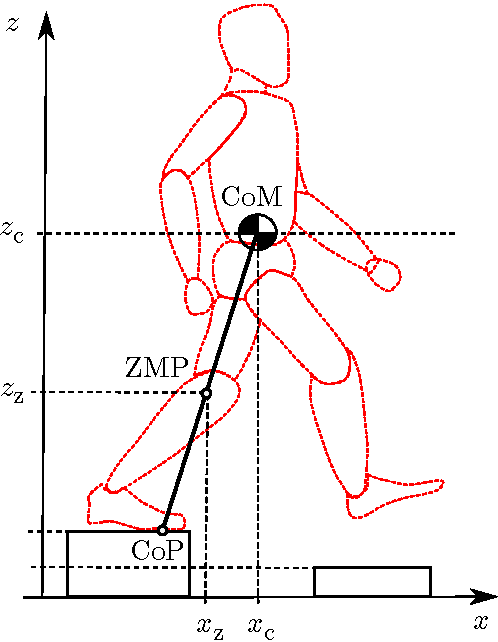
\includegraphics[width=0.45\textwidth]{figures/LIPM_robot.pdf}
    \caption{A humanoid walking under LIP dynamics. Note the positions of the CoM, the ZMP and the CoP, which lie on the same axis because of the assumption of conservation of angular momentum.}
    \label{fig:LIPM-robot}
\end{figure}

When walking on flat floor (a single contact surface with normal
$\bm{e}_z=(0 \; 0\; 1)^T$),
a common choice is to constrain the ZMP to lie on
a plane which coincides with the ground (i.e., without loss of generality
$z_Z=0$). As a consequence, the CoM is constrained to lie on a parallel plane
displaced by $h$ from the ZMP plane (i.e., $z_C=h$), and
the LIP dynamics further simplifies to the following dynamics:
\begin{align*}
    \ddot{x}_C &= \eta^2 (x_C - x_Z) \\
    \ddot{y}_C &= \eta^2 (y_C - y_Z).
\end{align*}
Note that, in this particular case, the ZMP coincides with the center of
pressure (CoP), which is the point of application of the contact force
$\bm{f}^{\mathrm{c}}$ on the ground \cite{SardainBessonnet2004}.

\section{Contact equilibrium}
%We are interested in defining the condition of equilibrium of a humanoid robot.
%As already stated in eq. \eqref{eq:feasible-contact-force}, a contact force
%$\bm{f}_k$ is feasible if it lies in the friction cone $\mathcal{C}_k$.
%Friction cones can be linearized by friction pyramids \cite{Caron2015RSS},
%obtaining a linear constraint on the contact forces. This constraint can be
%described in halfspace representation as
%\begin{equation}
%    \label{eq:friction-pyramid-halfspace}
%    \bm{F}_k \bm{f}_k \le \bm{0}.
%\end{equation}
%
%As explained in \cite{Caron2015RSS}, friction pyramid constraints can be used
%to compute the \textit{Contact Wrench Cone} (CWC), which can be described in
%halfspace representation as:
%\begin{equation*}
%    \bm{A}_O \bm{w}_O \le \bm{0}.
%\end{equation*}
%
%The CWC provides a necessary and sufficient condition for contact equilibrium of
%motions of the humanoid. Indeed, $\bm{w}_O$ belongs to the CWC if and only if
%there exists a set of contact forces $\{ \bm{f}_k \}$ which satisfy the
%centroidal dynamics equation \eqref{eq:centroidal-dynamics},
%the \textit{contact wrench} \eqref{eq:contact-wrench} and the friction pyramid
%constraints \eqref{eq:friction-pyramid-halfspace}.

We are interested in defining the condition of equilibrium of a humanoid robot.
While there exists a general condition on contact
equilibrium based on contact wrench cone \cite{Caron2015RSS}, in this manuscript
we assume that the friction coefficient defined in
\eqref{eq:feasible-contact-force} is sufficiently large to avoid slipping at the
contact surfaces.

This hypothesis allows us to focus on a simplified contact equilibrium
condition, which is relatively easy to deal with when developing a locomotion
scheme. In particular, consider the case of LIP dynamics of eq. \eqref{eq:LIPM}
with all contact forces directed towards the CoM, as described in
\cite{Sugihara2002ICRA}.
In this case, the contact forces can be rewritten as
\begin{equation}
    \label{eq:contact-force-towards-com}
    \bm{f}_k = \frac{\bm{p}_C - \bm{p}_k}{\| \bm{p}_C - \bm{p}_k \|_2} f_k,
\end{equation}
with $f_k$ the norm of $\bm{f}_k$. By plugging eq.
\eqref{eq:contact-force-towards-com} into eq.
\eqref{eq:centroidal-dynamics}, we obtain
\begin{equation}
    m \ddot{\bm{p}}_C = m \bm{g} + \sum_{k=1}^K \frac{\bm{p}_C - \bm{p}_k}{\| \bm{p}_C - \bm{p}_k \|_2} f_k.
\end{equation}
Moreover, using the dynamics of eq. \eqref{eq:LIPM}, we can obtain
obtain (after rearranging the terms), the following:
\begin{equation*}
    \bm{p}_Z = \bm{p}_C - \sum_{k=1}^K \frac{\bm{p}_C - \bm{p}_k}{\| \bm{p}_C - \bm{p}_k \|_2} \frac{f_k}{m \eta^2}.
\end{equation*}

Because of the assumption of sufficient joint torque actuation made in Sec.
\ref{sec:lagrangian-dynamics}, in principle, we could modulate $f_k$ to position
the ZMP within the area defined by the following set:
\begin{equation}
    \mathcal{S}_Z = \left\{ \bm{p}_Z \,\middle\vert\, \bm{p}_Z = \bm{p}_C + \sum_{k=1}^K \gamma_k (\bm{p}_k - \bm{p}_C), \; \gamma_k > 0  \right\},
\end{equation}
which is a polyhedral cone with apex $\bm{p}_C$, and
is known in literature as \textit{supporting region} \cite{Sugihara2021ICRA},
as it contains all feasible positions of the ZMP.

Despite the above hypothesis on contact forces seems a strong assumption, it
has been used successfully for both walking and running tasks
\cite{Sugihara2002ICRA,Zamparelli2018SYROCO,Sugihara2021ICRA,Smaldone2022Running}. Moreover, when in
single support (or when all contacts are coplanar), the above condition is
always satisfied if $\dot{\bm{L}}_C=\bm{0}$
\cite{Caron2017DynamicWalkingOverRoughTerrains}.